\documentclass{rdl}

\begin{document}


% \maketitle{Number}{Hand-In date}{Tutor names}{Group number}{Name of the first group member}{Name of the second group member}{Name of the third group member}{Name of the fourth group member}
\maketitle{1}{\today}{Andreas Bresser, Pierre Willenbrock}{0}{Student 1}{Student 2}{Student 3}{Student 4}

\section{Our answer to a worksheet!}
\label{sec:bringup}

\subsection{This is a subsection}

Here we have some normal text.

\begin{lstlisting}[language=bash,basicstyle=\footnotesize]
# And now a bash command for example to run roscore:
$ roscore
\end{lstlisting}

\ldots or how about some python code:

\begin{lstlisting}[language=python,basicstyle=\footnotesize]
print("Hello, world!")
\end{lstlisting}

\subsection{Tables}

And a basic table.
\begin{table}[h!]
  \begin{tabular}{|l|l|}
   \hline
   u & Steer to the left. \\ \hline
   i & \ldots \\
   \hline
  \end{tabular}
  \caption{Example table for steering commands}
  \label{tab:steering}
\end{table}

\subsection{Pictures!}
Here is a picture of the turtlebot robot:

\begin{figure}[h!]  % use h! to force the picture here, otherwise it might move to the next page
  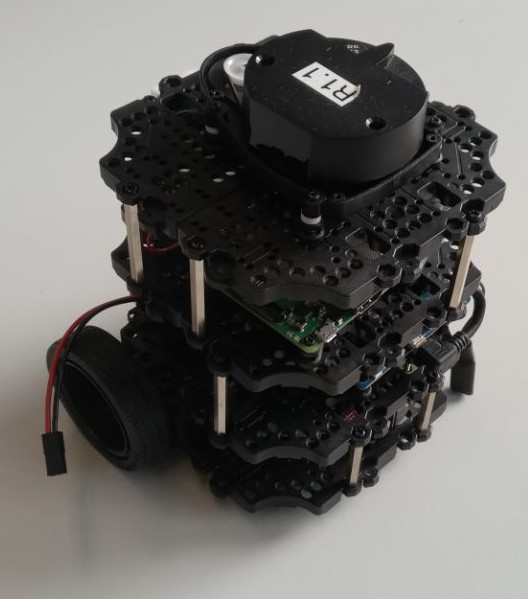
\includegraphics[width=0.25\linewidth]{picture/turtlebot.jpg}
  \caption{Turtelbot 3 burger.}
  \label{fig:turtlebot}
\end{figure}

The page is already full, let's force a page break!
\newpage 

\section{Bullet points}
\label{sec:quiz}

How about some Points?

\begin{itemize}
  \item First.
  \item Second.
  \item Third!
\end{itemize}

And don't forget that if you have something interesting to add you can also add a footnote.\footnote{Like this, you could add a reference to the source of your answer here for example, in a scientific paper you would manage your references in bibtex, and use "\textbackslash cite" but for worksheets a footonote is enough.}

You could upload all files to \url{https://overleaf.com} to work together on one document, but make sure you don't share it width other students outside of your group!

Even if you don't use overleaf, we recommend the \LaTeX\ documentation at \url{https://www.overleaf.com/learn/latex/}

\end{document}